\newpage
МРНТИ 52.45.19
\hfill {\bfseries \href{https://doi.org/10.58805/kazutb.v.3.24-480}{https://doi.org/10.58805/kazutb.v.3.24-480}}

\sectionwithauthors{А.Р. Мамбеталиева, Г.К. Макашева, Т.Ш. Тусупбекова, С. К. Калиаскаров, С. Сагатбек}{ВЛИЯНИЕ УЛЬТРАТОНКОГО ИЗМЕЛЬЧЕНИЯ НА ТЕХНОЛОГИЧЕСКИЕ ПОКАЗАТЕЛИ
ОБОГАЩЕНИЯ ОТВАЛЬНЫХ ХВОСТОВ}

\begin{center}
{\bfseries \textsuperscript{1}А.Р. Мамбеталиева, \textsuperscript{1}Г.К. Макашева\envelope,\textsuperscript{1} Т.Ш. Тусупбекова, \textsuperscript{2}С. К. Калиаскаров, \\\textsuperscript{2}С. Сагатбек}

\textsuperscript{1}Satbayev University, Алматы, Казахстан,

\textsuperscript{2}ТОО «КазГидроМедь»,Караганда, Казахстан
\end{center}
\envelope Корреспондент-автор: mguldanka@mail.ru


Проблемы, с которым приходится сталкиваться горнодобывающей
промышленности для достижения утилизации отвальных хвостов в
соответствии с принципами экономики замкнутого цикла, включает в себя
улучшение довольно ограниченных знаний о минералогии, концентрации
примесей и объём хвостов в хвостохранилищах. Также необходимо разработка
технологий, чтобы сделать процесс экономически целесообразным. Для
улучшения показателей операции измельчения и оказать существенное
влияние на обогащение ценных компонентов было изучена влияния
ультратонкого измельчения на степень раскрываемости медных минералов
отвальных хвостов.

На основании оптико-минералогических исследований установлено, что
абсолютно раскрытые зерна халькопирита составляют не более 35 \% от
общего количества зерен, их размер в основном (на 60 \% отн.) в пределах
класса 10-45 мкм. Анализ ситовых характеристик хвостов после
ультратонкого измельчения показывает, что наибольшая концентрация меди
приходится на самый тонкий класс -0,006+0 мм, что свидетельствует о
высоком раскрытии медных минералов за счет ультратонкого измельчения.
Флотационные тесты по определению влияния степени ультратонкого
измельчения показала, что с увеличением тонины помола по классу
крупности -- 0,045 + 0 мм до 86 \% повышается извлечения меди с 66,49 до
73,52 \%; золота 71,07 до 77,78 \%; серебро 70,29 до 76,71 \%.

{\bfseries Ключевые слова:} обогащение полезных ископаемых, флотация,
ультратонкое измельчения, отвальные хвосты, халькопирит,
минералогический анализ.

\sectionheading{УЛЬТРА ҰСАҚ ҰНТАҚТАУДЫҢ ҮЙІНДІ ҚАЛДЫҚТАРДЫҢ БАЙЫТУДЫҢ
ТЕХНОЛОГИЯЛЫҚ КӨРСЕТКІШТЕРІНЕ ӘСЕРІ}

\begin{center}
{\bfseries \textsuperscript{1}А.Р. Мамбеталиева, \textsuperscript{1}Г.К.
Макашева\envelope,\textsuperscript{1} Т.Ш. Тусупбекова,
\textsuperscript{2}С. К. Калиаскаров,}

{\bfseries \textsuperscript{2}С. Сагатбек}

\textsuperscript{1}Satbayev University, Алматы, Қазахстан,

\textsuperscript{2}«ҚазГидроМедь» ЖШС,Қарағанды, Қазахстан,

e-mail: mguldanka@mail.ru;
\end{center}

Айналмалы экономика қағидаларына сәйкес үйінді қалдықтарды кәдеге
жаратуға қол жеткізу үшін тау-кен өнеркәсібінің алдында тұрған мәселелер
минералогия, қоспалардың концентрациясы және қалдық қоймаларындағы
қалдықтардың көлемі туралы шектеулі білімді жақсартуды қамту қажет.
Процесті экономикалық тұрғыдан тиімді ету үшін технологияны дамыту
қажет. Ұнтақтау операциясының көрсеткіштерін жақсарту және құнды
компоненттерді байытуға айтарлықтай әсер ету үшін ультра жұқа
ұнтақтаудың үйінді қалдықтарының мыс минералдарының ашылу дәрежесіне
әсері зерттелді.

Оптикалық-минералогиялық зерттеулер негізінде мүлдем ашылған халькопирит
дәндері дәндердің жалпы санының 35\% - дан аспайтыны, олардың мөлшері
негізінен (60\% - ға) құрайтыны анықталды.) 10-45 мкм класс шегінде.
Ультра жұқа ұнтақтаудан кейін құйрықтардың елеуіш сипаттамаларын талдау
мыстың ең жоғары концентрациясы -0,006+0 мм ең жұқа класқа жататынын
көрсетеді, бұл ультра жұқа ұнтақтау арқылы мыс минералдарының жоғары
ашылуын көрсетеді. Ультра ұсақ ұнтақтау дәрежесінің әсерін анықтау
бойынша флотациялық сынақтар ұнтақтау тоннасының ұлғаюымен ұсақтау класы
бойынша -- 0,045 + 0 мм-ден 86\% - ға дейін мыс алу 66,49-дан 73,52\% -
ға дейін; алтын 71,07-ден 77,78\% - ға дейін; күміс 70,29-дан 76,71\% -
ға дейін артқанын көрсетті.

{\bfseries Түйін сөздер:} пайдалы қазбаларды байыту, флотация, ультра жұқа
ұнтақтау, үиінді қалдықтар, халькопирит, минералогиялық талдау.

\sectionheading{THE EFFECT OF ULTRAFINE GRINDING ON THE TECHNOLOGICAL PARAMETERS
OF THE ENRICHMENT OF DUMP TAILINGS}

\begin{center}
{\bfseries \textsuperscript{1}A.R. Mambetaliyeva, \textsuperscript{1}G.K.
Makasheva\envelope, \textsuperscript{1}T.Sh Tusupbekova,
\textsuperscript{2}S.K. Kaliaskarov,}

{\bfseries \textsuperscript{2}S. Sagatbek}

\textsuperscript{1}Satbayev University, Almaty, Kazakhstan,

\textsuperscript{2}Research Engineer at Kazhydromed LLP, Karaganda,
Kazakhstan,

e-mail: mguldanka@mail.ru;
\end{center}

The challenges that the mining industry has to face in order to achieve
tailings disposal in accordance with the principles of a closed-loop
economy include improving rather limited knowledge about mineralogy,
impurity concentrations and tailings volume in tailings dumps. It is
also necessary to develop technologies to make the process economically
feasible. In order to improve the performance of the grinding operation
and have a significant impact on the enrichment of valuable components,
the effects of ultrathin grinding on the degree of disclosure of copper
minerals of dump tailings were studied.

Based on optical and mineralogical studies, it was found that the
completely uncovered chalcopyrite grains make up no more than 35\% of
the total number of grains, their size is mainly (by 60\% relative)
within the class of 10-45 microns. Analysis of the sieve characteristics
of the tailings after ultrathin grinding shows that the highest
concentration of copper falls on the thinnest class -0.006+0 mm, that
indicates a high disclosure of copper minerals due to ultrathin
grinding. Flotation tests to determine the effect of the degree of
ultrathin grinding showed that with an increase in the fineness of
grinding in the size class -- 0.045 + 0 mm to 86\%, the extraction of
copper increases from 66.49 to 73.52\%; gold 71.07 to 77.78\%; silver
70.29 to 76.71\%.

{\bfseries Keywords:} mineral processing, flotation, ultra-fine grinding,
waste tailings, chalcopyrite, mineralogical analysis.

\begin{multicols}{2}
{\bfseries Введение.} В настоящее время измельчение играет жизненно важную
роль в различных областях, включая горнодобывающую, химическую,
цементную и строительную промышленность. Для обогащения полезных
ископаемых подготовительным является измельчение, целью которого
является завершение мономерного отделения ценных минералов от пустых, и
получение квалифицированного материала для дальнейшего обогащения
{[}1{]}. Технологическая производительность измельчения фактически
определяет производительность обогащения и качество продуктов, тем самым
напрямую влияя на показатель содержания концентрата {[}2{]}. По
сравнению со стальной шаровой средой, керамическая шаровая среда
обладает характеристиками хорошей износостойкости, высокой твердости и
низкой плотности, и, таким образом, может значительно снизить расход
мощности измельчения и мелющих тел при применении в мельницах с
перемешиванием мелющей среды {[}1,3,{]}. Кроме того, керамическая
шаровая среда может улучшить флотационные характеристики цветных и
благородных руд за счет восстановления ионов железа, образующихся при
измельчении {[}4{]}. Следовательно, улучшение показателей операции
измельчения может оказать существенно влияние на обогащение полезных
ископаемых.

По мере истощения крупнозернистых, легко перерабатываемых рудных тел
перерабатываются более вкрапленные, мелкозернистые руды. Адекватное
высвобождение ценных компонентов в мелкозернистой руде часто достигается
только после того, как размер частиц руды был уменьшен до уровня ниже
традиционной границы шаровой мельницы в 45 мкм {[}5{]}.

Процесс ультратонкого измельчения заключается в получении ультрамельких
частиц руды. Единого стандарта для размера ультрадисперсных частиц не
существует, но принято считать, что ультрадисперсные частицы
металлической руды составляют менее 10 мкм, а неметаллической руды --
менее 5 мкм {[}6{]}.

Актуальность утилизации отвальных хвостов и хвостохранилищ заключается в
следующем, что в настоящее время наблюдается общемировая тенденция --
переход к «sustainable mining» (устойчивым геотехнологиям), одним из
направлений которых является расширение использования техногенных
отходов {[}7,8,{]}.

Недавние исследования показали, что переработка отвальных хвостов
является выгодной при одновременном снижении воздействия горнодобывающей
промышленности {[}9{]}. Так же разработаны исследования по изучению
методов обогащения, а именно флотации для переработки лежалых медных
хвостов {[}10{]}. Кроме того, с экономической точки зрения переработка
отходов используется как способ повышения эффективности использования
ресурсов {[}11{]} или перехода к безотходному процессу.

Основной целью данной работы является изучение влияния ультратонкого
измельчения в целях разработки технологии вторичной переработки лежалых
хвостов Карагайлинской обогатительной фабрики с получением сырья,
пригодного для дальнейшей переработки.

{\bfseries Материалы и методы.} Объект исследования -- проба лежалых
отвальных хвостов Карагайлинской обогатительной фабрики, за
складированных в карьере «Главный».

Вещественный состав пробы определялся масс-спектральным анализом с
индуктивно связанной плазмой (ICP-MS), содержание золота и серебра -
пробирным анализом. Согласно результатам химического анализа, содержание
основных ценных компонентов составило: меди 0,23 \%, серебра 8,11 г/т,
золота 0,78 г/т, цинка 0,35 \%, свинца 0,10 \%.

Изучение рудных минералов проводилось в отраженном свете в полированных
аншлифах-брикетах, с применением микроскопа OLYMPUS BX 53, видеокамеры
SIMAGIS XS-3CU и программного обеспечения для анализа изображений
Минерал С7 компании SIAMS.

На основании оптико-минералогических исследований установлено, что в
минеральном составе пробы преобладают породообразующие минералы, общее
содержание которых составляет 78,85 \%.

Рудные минералы распределяются следующим образом:

\begin{itemize}
\item
  основной (преобладающий) − пирит (20 \%):
\item
  второстепенные − сфалерит (0,5 \%), халькопирит (0,35 \%);
\item
  редкие или единичные знаки − оксиды железа (ред. зн.), ковеллин (ред.
  зн.), гидроокислы железа (ед. зн.), галенит (ед. зн.), блеклые руды
  (ред. зн.):
\item
  минералы благородных металлов в пробе не визуализированы.
\end{itemize}

Халькопирит (0,35 \% абс.) является основной минеральной формой
нахождения меди в пробе. Образует как самостоятельные отдельности (см.
рисунок 1a), так и сростки с нерудными минералами (см. рисунок 1b),
сфалеритом и пиритом. В сфалерите образует эмульсионные включения
(рисунок 1с). В пирите выполняет трещинки катаклаза или встречается в
виде тонких пойкилитовых включений (см. рисунок 2d), иногда в тесной
ассоциации с блеклыми рудами.

Присутствие халькопирита в тесной ассоциации с пиритом, в том числе в
виде тонких включений может отрицательно сказываться на показателях
обогащения и на селективном выделении данных компонентов руды.

Абсолютно раскрытые зерна халькопирита составляют не более 35 \% от
общего количества зерен, их размер в основном (на 60 \% отн.) в пределах
класса 10-45 мкм.

Проведены исследования с использованием сверхтонкого измельчения в
лабораторной бисерной мельнице (далее МБЛ-1) по определению кинетики
измельчения исходной пробы отвальных хвостов контролем крупности
исходного продукта.
\end{multicols}

\begin{figure}[H]
    \centering
    \begin{subfigure}[b]{0.45\textwidth}
        \centering
        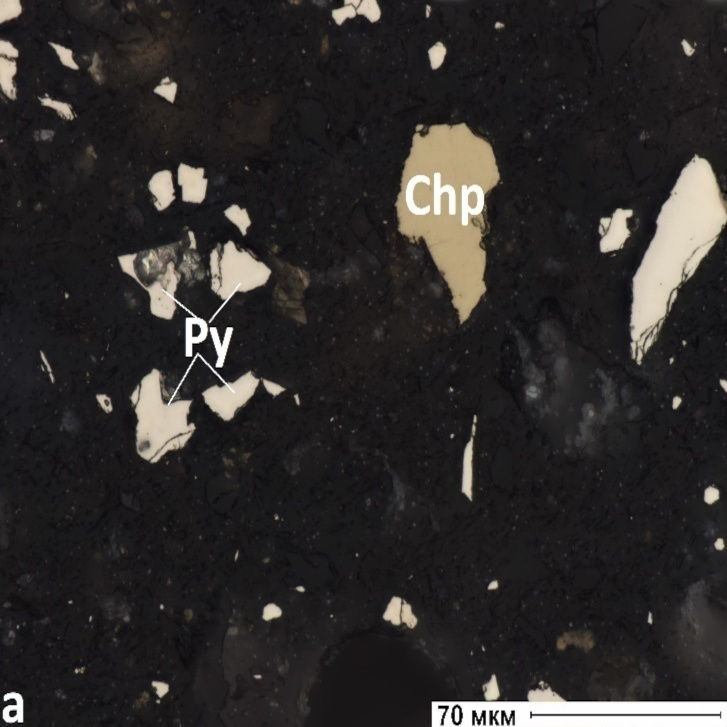
\includegraphics[width=\textwidth]{assets/296}
    \end{subfigure}
    \begin{subfigure}[b]{0.45\textwidth}
        \centering
        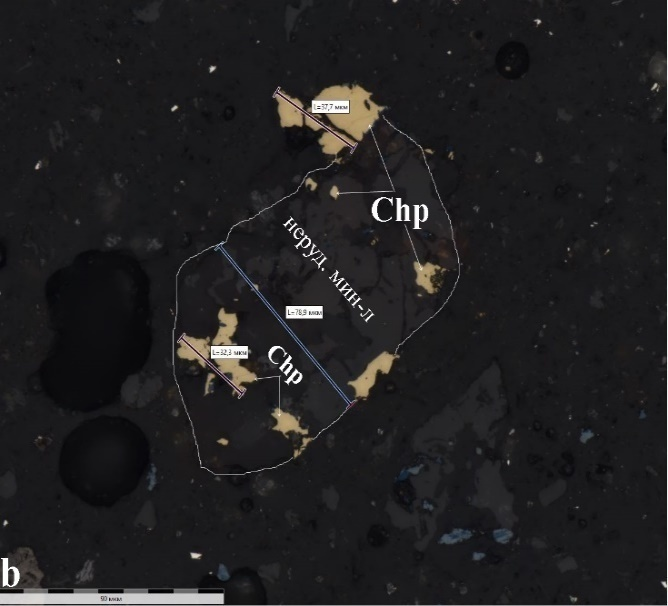
\includegraphics[width=\textwidth]{assets/297}
    \end{subfigure}
    \begin{subfigure}[b]{0.45\textwidth}
        \centering
        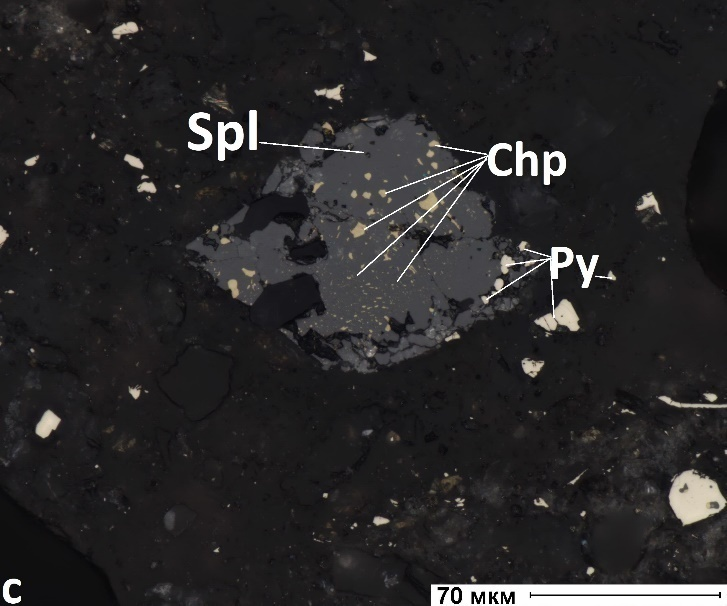
\includegraphics[width=\textwidth]{assets/298}
    \end{subfigure}
    \begin{subfigure}[b]{0.45\textwidth}
        \centering
        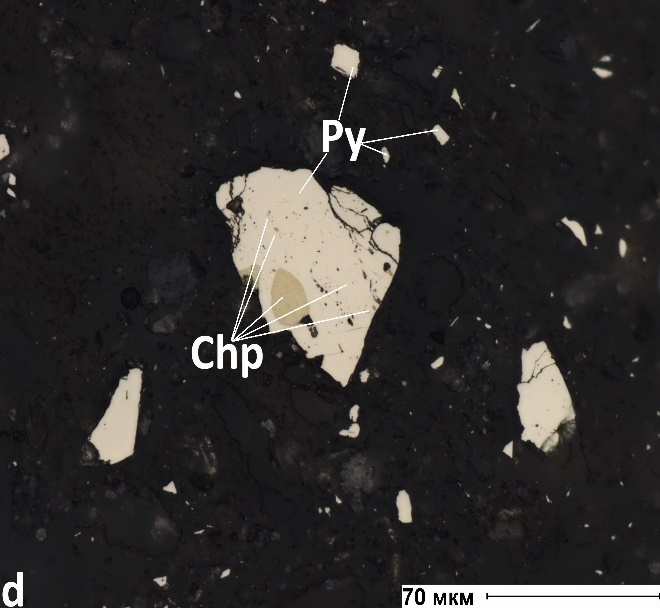
\includegraphics[width=\textwidth]{assets/299}
    \end{subfigure}
    \caption*{\normalfont Chp-халькопирит, Spl-сфалерит, Py-пирит.}
    \caption*{Рис. 1 -- Характеристика выделений халькопирита. Увел. 200/500}
\end{figure}

\begin{multicols}{2}
Известно, что использование тонкого и сверхтонкого помола продуктов,
содержащих благородные металлы, значительно увеличивает извлечение
золота и серебра в процессе обогащения. Но возможность моделирования
процесса измельчения в непрерывном режиме для бисерной мельницы является
основной проблемой на данный момент.

На рынке лабораторного оборудования представлен широкий ассортимент
лабораторных бисерных мельниц, зарубежных компании, среди разработок в
России -- это мельница МПБ -- 1 совместного российского-казахстанского
производства ТОО «SMAK Technology» и ООО БФК «Инжиниринг».

Лаборатории ООО "БФК Инжиниринг" и полупромышленные бисерные мельницы
имеют возможность моделировать технологический процесс ультратонкого
измельчения в поточном режиме {[}12{]}.

Внешний вид мельницы показаны на рисунке 2.
\end{multicols}

\begin{figure}[H]
	\centering
	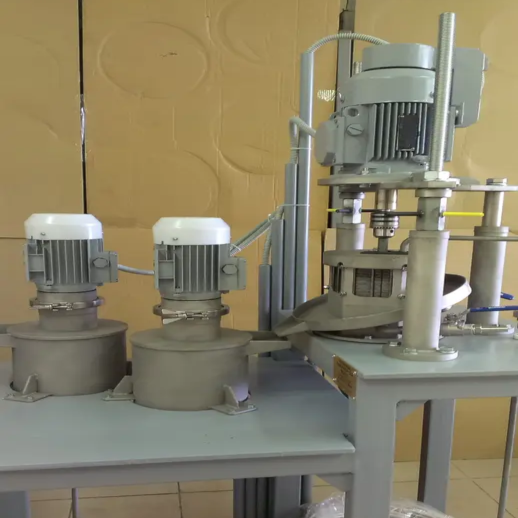
\includegraphics[width=0.7\textwidth]{assets/300}
	\caption*{Рис. 2 -- Внешний вид бисерной мельницы МБЛ -- 1 для
сверхтонкого измельчения}
\end{figure}

\begin{multicols}{2}
Флотационное обогащение выполнялось на стандартных лабораторных
пневмомеханических флотационных машинах типа Вэктис с объемом камер 3,
1.0 и 0.5 л.

Для исследования были применены следующие реагенты:

- сернистый натрий -- активатор;

- ксантогенат бутиловый - собиратель;

- МИБК -- пенообразователь;

Из вышеперечисленных реагентов приготавливались растворы необходимой
концентрации, с пересчетом на 100 \% активность, по формуле:

\[P = \frac{V \cdot C}{A};\]

где V -- объем воды, мл; А -- активность, \%; C -- концентрация
реагента, д.е;

{\bfseries Результаты и обсуждение.} Результаты определения кинетики
измельчения исходной пробы хвостов c контролем крупности исходного
продукта представлены в таблице 1.
\end{multicols}

{\small
\begin{longtable}[c]{|p{0.15\textwidth}ccccccccccc|}
\caption*{Таблица 1 -- Кинетика измельчения отвальных хвостов обогащения} \\
\hline
\multicolumn{1}{|p{0.15\textwidth}|}{\multirow{2}{=}{Наименование продуктов, мм}} & \multicolumn{1}{p{0.06\textwidth}|}{\multirow{2}{=}{Выход, \%}} & \multicolumn{5}{l|}{Содержание, \%} & \multicolumn{5}{l|}{Распределение, \%} \\ \cline{3-12} 
\multicolumn{1}{|c|}{} & \multicolumn{1}{c|}{} & \multicolumn{1}{c|}{Cu} & \multicolumn{1}{c|}{Fe} & \multicolumn{1}{c|}{S} & \multicolumn{1}{c|}{Au} & \multicolumn{1}{c|}{Ag} & \multicolumn{1}{c|}{Cu} & \multicolumn{1}{c|}{Fe} & \multicolumn{1}{c|}{S} & \multicolumn{1}{c|}{Au} & Ag \\ \hline
\endfirsthead
%
\endhead
%
\multicolumn{12}{|c|}{Исходная проба} \\ \hline
\multicolumn{1}{|c|}{0,071} & \multicolumn{1}{c|}{16,91} & \multicolumn{1}{c|}{0,17} & \multicolumn{1}{c|}{5,39} & \multicolumn{1}{c|}{2,05} & \multicolumn{1}{c|}{0,37} & \multicolumn{1}{c|}{2,66} & \multicolumn{1}{c|}{12,48} & \multicolumn{1}{c|}{7,39} & \multicolumn{1}{c|}{3,11} & \multicolumn{1}{c|}{8,01} & 5,54 \\ \hline
\multicolumn{1}{|c|}{-0,071 + 0,045} & \multicolumn{1}{c|}{14,34} & \multicolumn{1}{c|}{0,18} & \multicolumn{1}{c|}{11,65} & \multicolumn{1}{c|}{10,75} & \multicolumn{1}{c|}{0,56} & \multicolumn{1}{c|}{5,67} & \multicolumn{1}{c|}{11,12} & \multicolumn{1}{c|}{13,55} & \multicolumn{1}{c|}{13,81} & \multicolumn{1}{c|}{10,23} & 10,03 \\ \hline
\multicolumn{1}{|c|}{-0,045 + 0,035} & \multicolumn{1}{c|}{12,07} & \multicolumn{1}{c|}{0,22} & \multicolumn{1}{c|}{17,69} & \multicolumn{1}{c|}{16,73} & \multicolumn{1}{c|}{1,2} & \multicolumn{1}{c|}{9,35} & \multicolumn{1}{c|}{11,33} & \multicolumn{1}{c|}{17,32} & \multicolumn{1}{c|}{18,09} & \multicolumn{1}{c|}{18,61} & 13,91 \\ \hline
\multicolumn{1}{|c|}{-0,035+0,025} & \multicolumn{1}{c|}{11,32} & \multicolumn{1}{c|}{0,26} & \multicolumn{1}{c|}{20,34} & \multicolumn{1}{c|}{19,47} & \multicolumn{1}{c|}{1,15} & \multicolumn{1}{c|}{10,83} & \multicolumn{1}{c|}{12,58} & \multicolumn{1}{c|}{18,67} & \multicolumn{1}{c|}{19,75} & \multicolumn{1}{c|}{16,73} & 15,12 \\ \hline
\multicolumn{1}{|c|}{-0,025+0,017} & \multicolumn{1}{c|}{6,47} & \multicolumn{1}{c|}{0,15} & \multicolumn{1}{c|}{16,18} & \multicolumn{1}{c|}{14,71} & \multicolumn{1}{c|}{0,95} & \multicolumn{1}{c|}{6,98} & \multicolumn{1}{c|}{4,29} & \multicolumn{1}{c|}{8,49} & \multicolumn{1}{c|}{8,53} & \multicolumn{1}{c|}{7,9} & 5,57 \\ \hline
\multicolumn{1}{|c|}{-0,017+0,008} & \multicolumn{1}{c|}{10,52} & \multicolumn{1}{c|}{0,15} & \multicolumn{1}{c|}{16,71} & \multicolumn{1}{c|}{14,88} & \multicolumn{1}{c|}{0,98} & \multicolumn{1}{c|}{8,63} & \multicolumn{1}{c|}{6,89} & \multicolumn{1}{c|}{14,26} & \multicolumn{1}{c|}{14,03} & \multicolumn{1}{c|}{13,21} & 11,19 \\ \hline
\multicolumn{1}{|c|}{-0,008+0,006} & \multicolumn{1}{c|}{1,25} & \multicolumn{1}{c|}{0,15} & \multicolumn{1}{c|}{15,49} & \multicolumn{1}{c|}{10,89} & \multicolumn{1}{c|}{0,99} & \multicolumn{1}{c|}{7,53} & \multicolumn{1}{c|}{0,82} & \multicolumn{1}{c|}{1,57} & \multicolumn{1}{c|}{1,22} & \multicolumn{1}{c|}{1,59} & 1,16 \\ \hline
\multicolumn{1}{|c|}{-0,006+0} & \multicolumn{1}{c|}{27,12} & \multicolumn{1}{c|}{0,34} & \multicolumn{1}{c|}{8,53} & \multicolumn{1}{c|}{8,83} & \multicolumn{1}{c|}{0,68} & \multicolumn{1}{c|}{11,21} & \multicolumn{1}{c|}{40,49} & \multicolumn{1}{c|}{18,75} & \multicolumn{1}{c|}{21,46} & \multicolumn{1}{c|}{23,72} & 37,48 \\ \hline
\multicolumn{1}{|c|}{Исходная проба} & \multicolumn{1}{c|}{100} & \multicolumn{1}{c|}{0,23} & \multicolumn{1}{c|}{12,33} & \multicolumn{1}{c|}{11,16} & \multicolumn{1}{c|}{0,78} & \multicolumn{1}{c|}{8,11} & \multicolumn{1}{c|}{100} & \multicolumn{1}{c|}{100} & \multicolumn{1}{c|}{100} & \multicolumn{1}{c|}{100} & 100 \\ \hline
\multicolumn{12}{|c|}{Время измельчения 5 мин} \\ \hline
\multicolumn{1}{|c|}{0,071} & \multicolumn{1}{c|}{10,61} & \multicolumn{1}{c|}{0,21} & \multicolumn{1}{c|}{4,87} & \multicolumn{1}{c|}{3,08} & \multicolumn{1}{c|}{0,28} & \multicolumn{1}{c|}{3,2} & \multicolumn{1}{c|}{9,76} & \multicolumn{1}{c|}{4,19} & \multicolumn{1}{c|}{2,93} & \multicolumn{1}{c|}{3,81} & 4,18 \\ \hline
\multicolumn{1}{|c|}{-0,071 + 0,045} & \multicolumn{1}{c|}{3,14} & \multicolumn{1}{c|}{0,47} & \multicolumn{1}{c|}{28,11} & \multicolumn{1}{c|}{30,14} & \multicolumn{1}{c|}{1,76} & \multicolumn{1}{c|}{18,34} & \multicolumn{1}{c|}{6,47} & \multicolumn{1}{c|}{7,16} & \multicolumn{1}{c|}{8,48} & \multicolumn{1}{c|}{7,09} & 7,1 \\ \hline
\multicolumn{1}{|c|}{-0,045 + 0,035} & \multicolumn{1}{c|}{12,01} & \multicolumn{1}{c|}{0,13} & \multicolumn{1}{c|}{15,27} & \multicolumn{1}{c|}{14,62} & \multicolumn{1}{c|}{1,02} & \multicolumn{1}{c|}{9,14} & \multicolumn{1}{c|}{6,96} & \multicolumn{1}{c|}{14,87} & \multicolumn{1}{c|}{15,73} & \multicolumn{1}{c|}{15,75} & 13,53 \\ \hline
\multicolumn{1}{|c|}{-0,035+0,025} & \multicolumn{1}{c|}{20,7} & \multicolumn{1}{c|}{0,2} & \multicolumn{1}{c|}{13,43} & \multicolumn{1}{c|}{12,7} & \multicolumn{1}{c|}{0,8} & \multicolumn{1}{c|}{7,71} & \multicolumn{1}{c|}{17,56} & \multicolumn{1}{c|}{22,54} & \multicolumn{1}{c|}{23,56} & \multicolumn{1}{c|}{21,11} & 19,68 \\ \hline
\multicolumn{1}{|c|}{-0,025+0,017} & \multicolumn{1}{c|}{5,47} & \multicolumn{1}{c|}{0,17} & \multicolumn{1}{c|}{12,44} & \multicolumn{1}{c|}{11,34} & \multicolumn{1}{c|}{0,75} & \multicolumn{1}{c|}{7,32} & \multicolumn{1}{c|}{4,07} & \multicolumn{1}{c|}{5,52} & \multicolumn{1}{c|}{5,56} & \multicolumn{1}{c|}{5,28} & 4,94 \\ \hline
\multicolumn{1}{|c|}{-0,017+0,008} & \multicolumn{1}{c|}{10,6} & \multicolumn{1}{c|}{0,16} & \multicolumn{1}{c|}{11,29} & \multicolumn{1}{c|}{10,01} & \multicolumn{1}{c|}{0,7} & \multicolumn{1}{c|}{6,2} & \multicolumn{1}{c|}{7,22} & \multicolumn{1}{c|}{9,71} & \multicolumn{1}{c|}{9,51} & \multicolumn{1}{c|}{9,46} & 8,11 \\ \hline
\multicolumn{1}{|c|}{-0,008+0,006} & \multicolumn{1}{c|}{0,49} & \multicolumn{1}{c|}{0,16} & \multicolumn{1}{c|}{10,06} & \multicolumn{1}{c|}{7,98} & \multicolumn{1}{c|}{0,73} & \multicolumn{1}{c|}{5,47} & \multicolumn{1}{c|}{0,34} & \multicolumn{1}{c|}{0,4} & \multicolumn{1}{c|}{0,35} & \multicolumn{1}{c|}{0,46} & 0,33 \\ \hline
\multicolumn{1}{|c|}{-0,006+0} & \multicolumn{1}{c|}{36,98} & \multicolumn{1}{c|}{0,3} & \multicolumn{1}{c|}{11,87} & \multicolumn{1}{c|}{10,22} & \multicolumn{1}{c|}{0,78} & \multicolumn{1}{c|}{9,24} & \multicolumn{1}{c|}{47,62} & \multicolumn{1}{c|}{35,61} & \multicolumn{1}{c|}{33,88} & \multicolumn{1}{c|}{37,04} & 42,13 \\ \hline
\multicolumn{1}{|c|}{Исходная проба} & \multicolumn{1}{c|}{100} & \multicolumn{1}{c|}{0,23} & \multicolumn{1}{c|}{12,33} & \multicolumn{1}{c|}{11,16} & \multicolumn{1}{c|}{0,78} & \multicolumn{1}{c|}{8,11} & \multicolumn{1}{c|}{100} & \multicolumn{1}{c|}{100} & \multicolumn{1}{c|}{100} & \multicolumn{1}{c|}{100} & 100 \\ \hline
\multicolumn{12}{|c|}{Время измельчения 10 мин} \\ \hline
\multicolumn{1}{|c|}{0,071} & \multicolumn{1}{c|}{8,6} & \multicolumn{1}{c|}{0,22} & \multicolumn{1}{c|}{3,64} & \multicolumn{1}{c|}{1,78} & \multicolumn{1}{c|}{0,35} & \multicolumn{1}{c|}{2,08} & \multicolumn{1}{c|}{8,1} & \multicolumn{1}{c|}{2,54} & \multicolumn{1}{c|}{1,37} & \multicolumn{1}{c|}{3,81} & 2,21 \\ \hline
\multicolumn{1}{|c|}{-0,071 + 0,045} & \multicolumn{1}{c|}{2,74} & \multicolumn{1}{c|}{0,35} & \multicolumn{1}{c|}{20,2} & \multicolumn{1}{c|}{20,69} & \multicolumn{1}{c|}{2,02} & \multicolumn{1}{c|}{12,11} & \multicolumn{1}{c|}{4,11} & \multicolumn{1}{c|}{4,49} & \multicolumn{1}{c|}{5,08} & \multicolumn{1}{c|}{7,09} & 4,09 \\ \hline
\multicolumn{1}{|c|}{-0,045 + 0,035} & \multicolumn{1}{c|}{5,97} & \multicolumn{1}{c|}{0,24} & \multicolumn{1}{c|}{15,26} & \multicolumn{1}{c|}{14,48} & \multicolumn{1}{c|}{2,06} & \multicolumn{1}{c|}{8,24} & \multicolumn{1}{c|}{6,26} & \multicolumn{1}{c|}{7,38} & \multicolumn{1}{c|}{7,74} & \multicolumn{1}{c|}{15,75} & 6,06 \\ \hline
\multicolumn{1}{|c|}{-0,035+0,025} & \multicolumn{1}{c|}{15,37} & \multicolumn{1}{c|}{0,21} & \multicolumn{1}{c|}{14,98} & \multicolumn{1}{c|}{14,61} & \multicolumn{1}{c|}{1,07} & \multicolumn{1}{c|}{8,72} & \multicolumn{1}{c|}{14,35} & \multicolumn{1}{c|}{18,67} & \multicolumn{1}{c|}{20,13} & \multicolumn{1}{c|}{21,11} & 16,52 \\ \hline
\multicolumn{1}{|c|}{-0,025+0,017} & \multicolumn{1}{c|}{4,82} & \multicolumn{1}{c|}{0,21} & \multicolumn{1}{c|}{14,79} & \multicolumn{1}{c|}{14,24} & \multicolumn{1}{c|}{0,86} & \multicolumn{1}{c|}{8,16} & \multicolumn{1}{c|}{4,34} & \multicolumn{1}{c|}{5,78} & \multicolumn{1}{c|}{6,15} & \multicolumn{1}{c|}{5,28} & 4,85 \\ \hline
\multicolumn{1}{|c|}{-0,017+0,008} & \multicolumn{1}{c|}{11,42} & \multicolumn{1}{c|}{0,17} & \multicolumn{1}{c|}{13,15} & \multicolumn{1}{c|}{12,28} & \multicolumn{1}{c|}{0,65} & \multicolumn{1}{c|}{7,39} & \multicolumn{1}{c|}{8,6} & \multicolumn{1}{c|}{12,18} & \multicolumn{1}{c|}{12,56} & \multicolumn{1}{c|}{9,46} & 10,4 \\ \hline
\multicolumn{1}{|c|}{-0,008+0,006} & \multicolumn{1}{c|}{0,52} & \multicolumn{1}{c|}{0,19} & \multicolumn{1}{c|}{11,99} & \multicolumn{1}{c|}{10,85} & \multicolumn{1}{c|}{0,69} & \multicolumn{1}{c|}{6,96} & \multicolumn{1}{c|}{0,42} & \multicolumn{1}{c|}{0,51} & \multicolumn{1}{c|}{0,51} & \multicolumn{1}{c|}{0,46} & 0,45 \\ \hline
\multicolumn{1}{|c|}{-0,006+0} & \multicolumn{1}{c|}{50,56} & \multicolumn{1}{c|}{0,24} & \multicolumn{1}{c|}{11,81} & \multicolumn{1}{c|}{10,25} & \multicolumn{1}{c|}{0,57} & \multicolumn{1}{c|}{8,89} & \multicolumn{1}{c|}{53,82} & \multicolumn{1}{c|}{48,45} & \multicolumn{1}{c|}{46,46} & \multicolumn{1}{c|}{37,04} & 55,42 \\ \hline
\multicolumn{1}{|c|}{Исходная проба} & \multicolumn{1}{c|}{100} & \multicolumn{1}{c|}{0,23} & \multicolumn{1}{c|}{12,33} & \multicolumn{1}{c|}{11,16} & \multicolumn{1}{c|}{0,78} & \multicolumn{1}{c|}{8,11} & \multicolumn{1}{c|}{100} & \multicolumn{1}{c|}{100} & \multicolumn{1}{c|}{100} & \multicolumn{1}{c|}{100} & 100 \\ \hline
\multicolumn{12}{|c|}{Время измельчения 20 мин} \\ \hline
\multicolumn{1}{|c|}{0,071} & \multicolumn{1}{c|}{5,33} & \multicolumn{1}{c|}{0,2} & \multicolumn{1}{c|}{3,71} & \multicolumn{1}{c|}{1,89} & \multicolumn{1}{c|}{0,25} & \multicolumn{1}{c|}{2,03} & \multicolumn{1}{c|}{4,52} & \multicolumn{1}{c|}{1,6} & \multicolumn{1}{c|}{0,9} & \multicolumn{1}{c|}{1,7} & 1,33 \\ \hline
\multicolumn{1}{|c|}{-0,071 + 0,045} & \multicolumn{1}{c|}{3,07} & \multicolumn{1}{c|}{0,37} & \multicolumn{1}{c|}{22,43} & \multicolumn{1}{c|}{23,69} & \multicolumn{1}{c|}{1,52} & \multicolumn{1}{c|}{13,17} & \multicolumn{1}{c|}{4,9} & \multicolumn{1}{c|}{5,58} & \multicolumn{1}{c|}{6,51} & \multicolumn{1}{c|}{5,97} & 4,98 \\ \hline
\multicolumn{1}{|c|}{-0,045 + 0,035} & \multicolumn{1}{c|}{3,58} & \multicolumn{1}{c|}{0,25} & \multicolumn{1}{c|}{15,83} & \multicolumn{1}{c|}{15,64} & \multicolumn{1}{c|}{0,99} & \multicolumn{1}{c|}{9,14} & \multicolumn{1}{c|}{3,95} & \multicolumn{1}{c|}{4,59} & \multicolumn{1}{c|}{5,01} & \multicolumn{1}{c|}{4,55} & 4,03 \\ \hline
\multicolumn{1}{|c|}{-0,035+0,025} & \multicolumn{1}{c|}{10,02} & \multicolumn{1}{c|}{0,21} & \multicolumn{1}{c|}{14,78} & \multicolumn{1}{c|}{14,45} & \multicolumn{1}{c|}{0,97} & \multicolumn{1}{c|}{7,93} & \multicolumn{1}{c|}{9,12} & \multicolumn{1}{c|}{12,01} & \multicolumn{1}{c|}{12,97} & \multicolumn{1}{c|}{12,47} & 9,8 \\ \hline
\multicolumn{1}{|c|}{-0,025+0,017} & \multicolumn{1}{c|}{3,67} & \multicolumn{1}{c|}{0,19} & \multicolumn{1}{c|}{14,19} & \multicolumn{1}{c|}{13,61} & \multicolumn{1}{c|}{0,95} & \multicolumn{1}{c|}{7,67} & \multicolumn{1}{c|}{3,03} & \multicolumn{1}{c|}{4,22} & \multicolumn{1}{c|}{4,47} & \multicolumn{1}{c|}{4,45} & 3,47 \\ \hline
\multicolumn{1}{|c|}{-0,017+0,008} & \multicolumn{1}{c|}{9,1} & \multicolumn{1}{c|}{0,16} & \multicolumn{1}{c|}{12,65} & \multicolumn{1}{c|}{11,65} & \multicolumn{1}{c|}{0,84} & \multicolumn{1}{c|}{6,63} & \multicolumn{1}{c|}{6,53} & \multicolumn{1}{c|}{9,34} & \multicolumn{1}{c|}{9,5} & \multicolumn{1}{c|}{9,82} & 7,44 \\ \hline
\multicolumn{1}{|c|}{-0,008+0,006} & \multicolumn{1}{c|}{0,63} & \multicolumn{1}{c|}{0,22} & \multicolumn{1}{c|}{12,06} & \multicolumn{1}{c|}{10,75} & \multicolumn{1}{c|}{0,81} & \multicolumn{1}{c|}{6,66} & \multicolumn{1}{c|}{0,61} & \multicolumn{1}{c|}{0,62} & \multicolumn{1}{c|}{0,61} & \multicolumn{1}{c|}{0,65} & 0,52 \\ \hline
\multicolumn{1}{|c|}{-0,006+0} & \multicolumn{1}{c|}{64,62} & \multicolumn{1}{c|}{0,24} & \multicolumn{1}{c|}{11,84} & \multicolumn{1}{c|}{10,37} & \multicolumn{1}{c|}{0,73} & \multicolumn{1}{c|}{8,59} & \multicolumn{1}{c|}{67,34} & \multicolumn{1}{c|}{62,03} & \multicolumn{1}{c|}{60,03} & \multicolumn{1}{c|}{60,39} & 68,42 \\ \hline
\multicolumn{1}{|c|}{Исходная проба} & \multicolumn{1}{c|}{100} & \multicolumn{1}{c|}{0,23} & \multicolumn{1}{c|}{12,33} & \multicolumn{1}{c|}{11,16} & \multicolumn{1}{c|}{0,78} & \multicolumn{1}{c|}{8,11} & \multicolumn{1}{c|}{100} & \multicolumn{1}{c|}{100} & \multicolumn{1}{c|}{100} & \multicolumn{1}{c|}{100} & 100 \\ \hline
\end{longtable}}

Зависимость выхода класса крупности минус 0,006 мм от времени
ультратонкого измельчения показан на рисунке 3.

\begin{figure}[H]
	\centering
	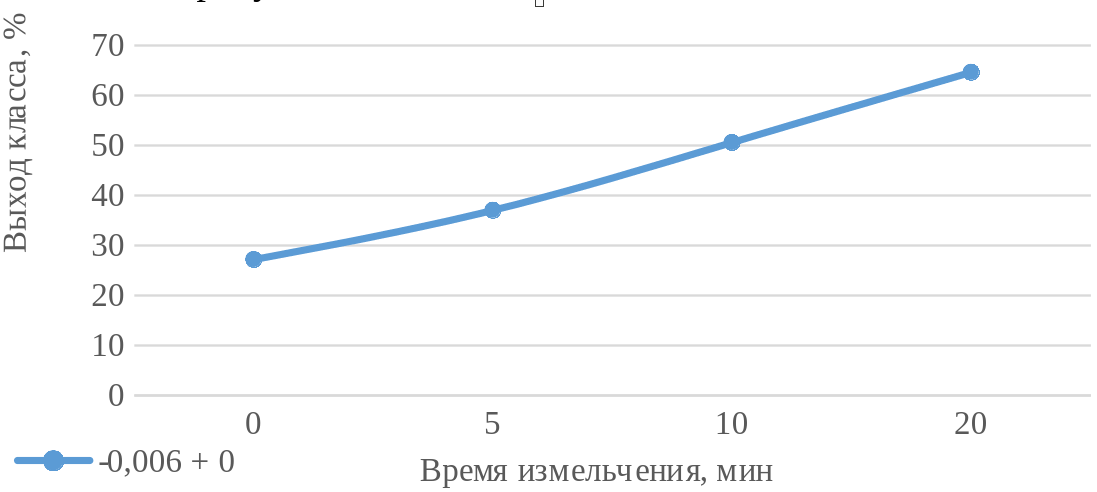
\includegraphics[width=0.8\textwidth]{assets/300.1}
	\caption*{Рис. 3 -- Зависимость выхода класса -0,006 мм от времени измельчения}
\end{figure}

\begin{multicols}{2}
Анализ ситовых характеристик хвостов после ультратонкого измельчения
показывает, что наибольшая концентрация меди приходится на самый тонкий
класс -0,006+0 мм, и повышается в зависимости от времени измельчения с
47,62 \% (5 минут) до 67.34 \% (20 минут), что свидетельствует о высоком
раскрытии медных минералов за счет ультратонкого измельчения. Однако,
увеличение выхода тонкого класса -0,006+0 мм с 27,12 \% в исходных
хвостах (см. таблицу 1) до 64,42 \% может отрицательно сказываться на
показателях обогащения, за счет ошламования процесса.

Кроме того, в тонких классах вместе с медью концентрируется и железо,
что подтверждает тесную связь минералов меди с пиритом, которую не
удается разрушить даже при ультратонком измельчении.

С целью определения влияния степени ультратонкого измельчения на
извлечение меди и благородных металлов выполнены флотационные тесты.

Схема проведения опыта указана на рисунке 4. Условия опытов приведены в
таблице 2; результаты представлены на рисунке 5-7.
\end{multicols}

\begin{figure}[H]
	\centering
	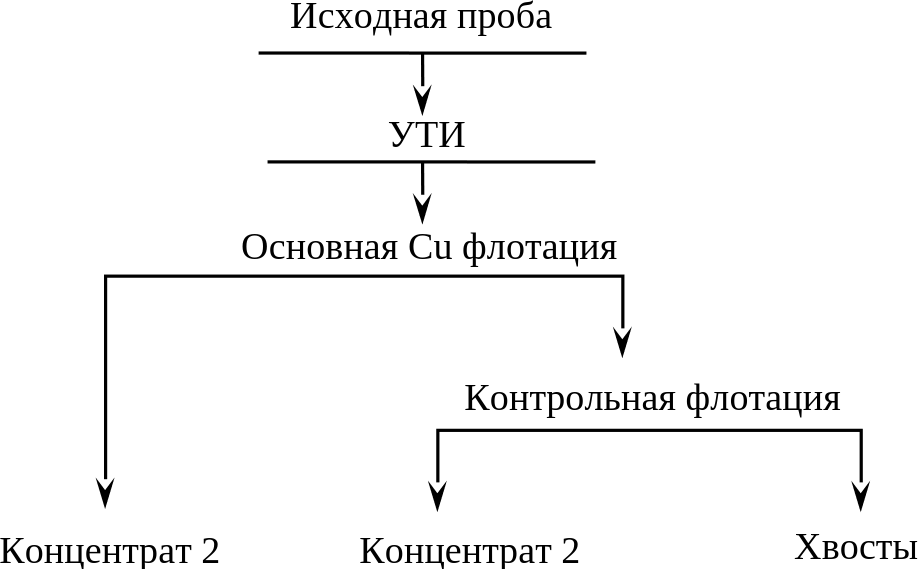
\includegraphics[width=0.4\textwidth]{assets/300.2}
	\caption*{Рис. 4 -- Лабораторная схема проведения опыта}
\end{figure}

\begin{figure}[H]
	\centering
	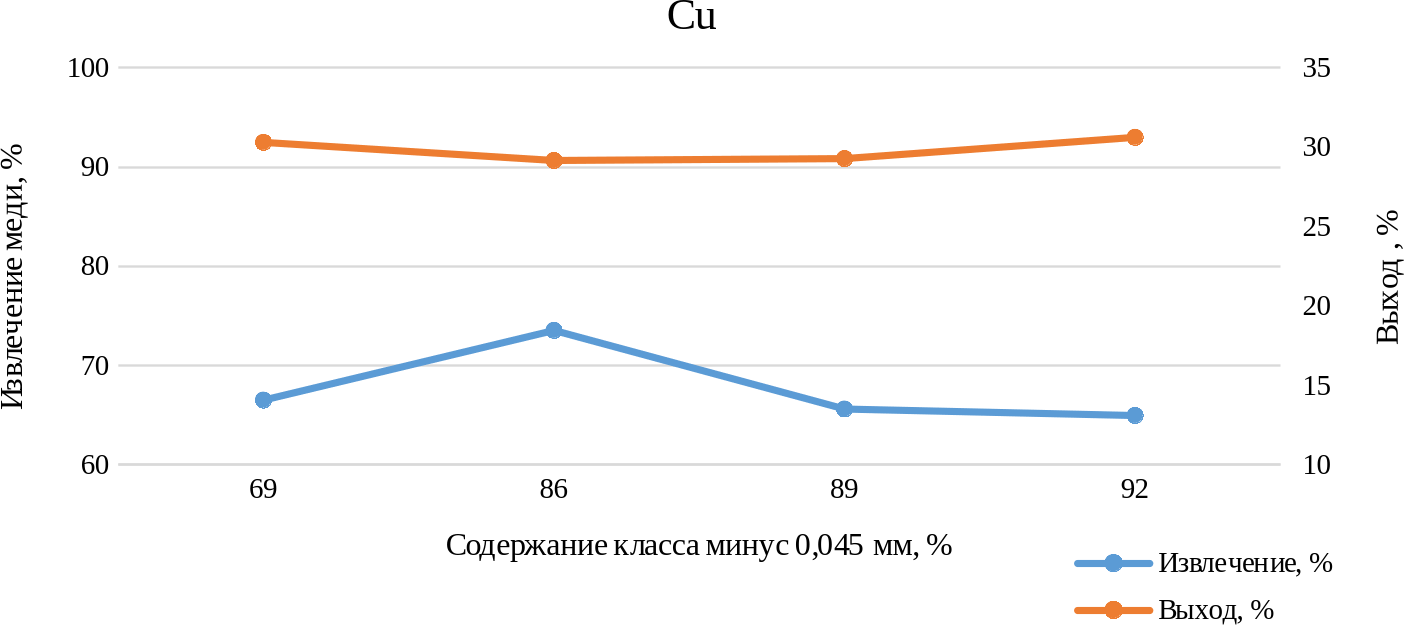
\includegraphics[width=0.83\textwidth]{assets/300.3}
	\caption*{Рис. 5 - Результаты тестов по подбору степени измельчения для
медных минералов}
\end{figure}

\begin{figure}[H]
	\centering
	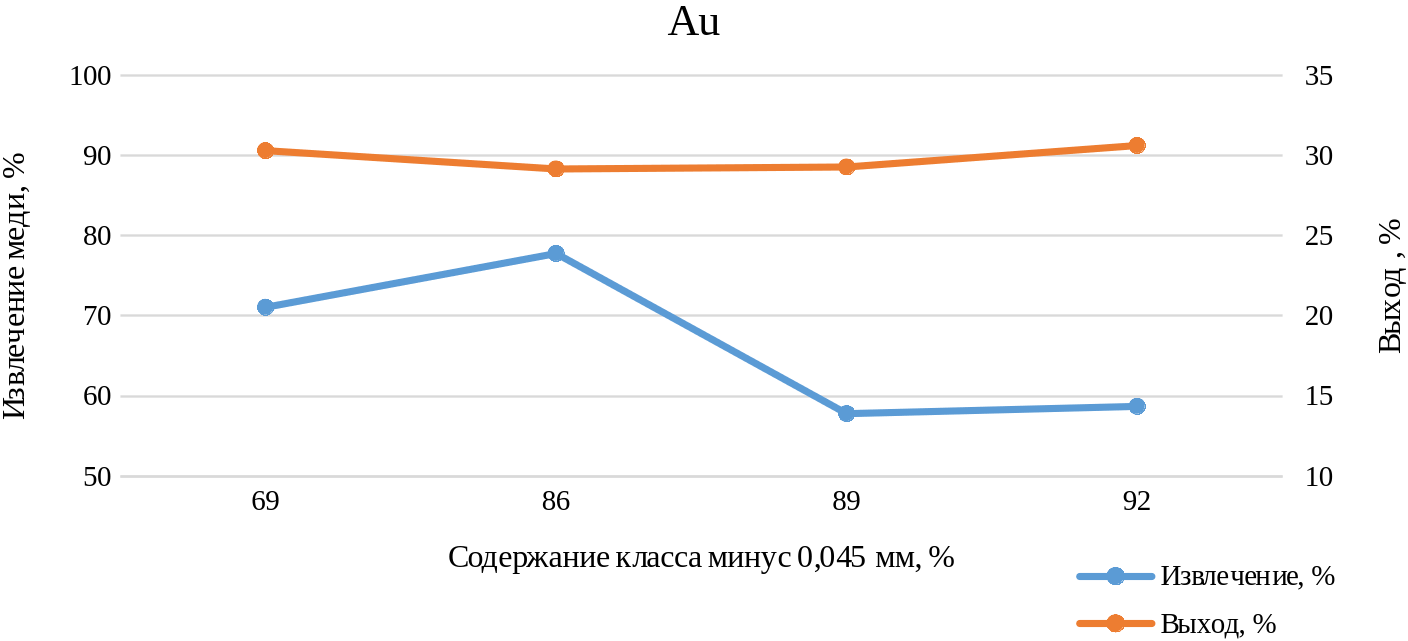
\includegraphics[width=0.83\textwidth]{assets/300.4}
	\caption*{Рис. 6 - Зависимость извлечения золота от степени измельчения
отвальных хвостов обогащения}
\end{figure}

\begin{figure}[H]
	\centering
	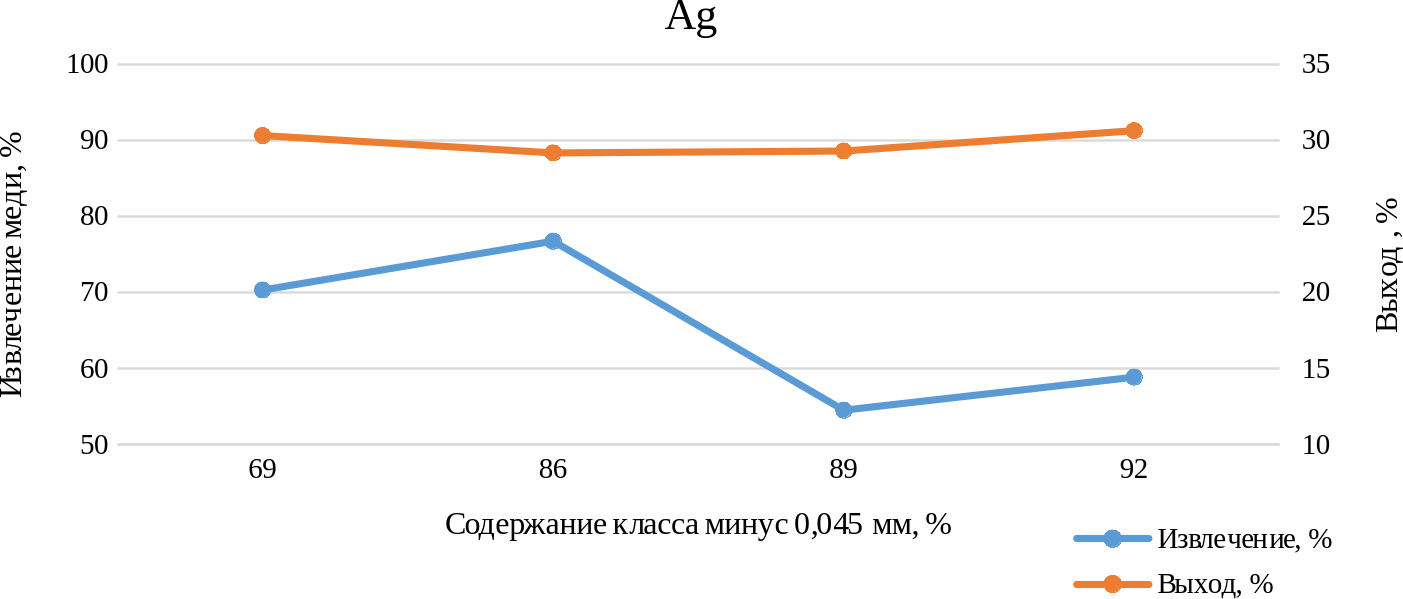
\includegraphics[width=0.83\textwidth]{assets/300.5}
	\caption*{Рис.7 - Зависимость извлечения серебра от степени измельчения
отвальных хвостов обогащения}
\end{figure}

\begin{table}[H]
\caption*{Таблица 2 -- Условия проведения опыта}
\centering
\begin{tabular}{|l|c|c|ccccc|c|}
\hline
\multirow{2}{*}{Операция} & \multirow{2}{*}{\begin{tabular}[c]{@{}l@{}}Время,\\   мин\end{tabular}} & \multirow{2}{*}{рН} & \multicolumn{5}{l|}{Расход реагентов, г/т} &  \\ \cline{4-9} 
 &  &  & \multicolumn{1}{c|}{МБС} & \multicolumn{1}{c|}{Na2S} & \multicolumn{1}{c|}{H2SO4} & \multicolumn{1}{c|}{Кх} & Aero 3418 & МИБК \\ \hline
\textbf{Всего:} & \textbf{-} & \textbf{-} & \multicolumn{1}{c|}{\textbf{800}} & \multicolumn{1}{c|}{\textbf{150}} & \multicolumn{1}{c|}{\textbf{7000}} & \multicolumn{1}{c|}{\textbf{100}} & \textbf{15} & \textbf{10} \\ \hline
Измельчение, -0,045 мм & 5,10,20 & - & \multicolumn{1}{c|}{800} & \multicolumn{1}{c|}{-} & \multicolumn{1}{c|}{-} & \multicolumn{1}{c|}{-} & - & - \\ \hline
Основная Cu флотация & 10 & 7,7 & \multicolumn{1}{c|}{-} & \multicolumn{1}{c|}{150} & \multicolumn{1}{c|}{-} & \multicolumn{1}{c|}{-} & 15 & 5 \\ \hline
Контрольная флотация & 10 & 3 & \multicolumn{1}{c|}{-} & \multicolumn{1}{c|}{-} & \multicolumn{1}{c|}{7000} & \multicolumn{1}{c|}{100} & - & 5 \\ \hline
\end{tabular}
\end{table}

\begin{multicols}{2}
Из рисунков 5-7 следует, что с увеличением тонины помола по классу
крупности -0,045+0 мм с 69 до 86 \% наблюдается повышение извлечения
меди в суммарном концентрате на 7,03 \% (66,49 до 73,52 \%), также
повышается извлечения благородных металлов, золота на 6,71 \% (71,07 до
77,78 \%), серебро на 6,42 \% (70,29 \% до 76,71 \%).

{\bfseries Выводы.} Для расширения сырьевой базы и комплексного
использования сырья Казахстана принято решение о необходимости
рассмотрении возможности вторичной переработки отвальных хвостов
Карагайлинской обогатительной фабрики, за складированных в карьере
«Главный».

Выделение ценных компонентов из мелкозернистых руд часто достигается
только после того, как размер частицы руды снижается до уровня ниже
порового значения традиционной шаровой мельницы в - 0,045 мм.

Проведены исследования с использованием сверхтонкого измельчения в
лабораторной бисерной мельнице (далее МБЛ-1) по определению кинетики
измельчения исходной пробы отвальных хвостов контролем крупности
исходного продукта.

Чтобы определить влияние степени сверхтонкого измельчения на извлечение
меди и благородных металлов, были проведены флотационные тесты.

Из результатов представленный в графике 5-7 следует, что оптимальный
тонины помола по классу крупности -- 0,045 +0 мм 86 \%, при это
наблюдается увлечения извлечения меди в суммарной концентрат на 73,52
\%, золота на 77,78 \%, серебро на 76,71 \%.
\end{multicols}

\begin{center}
{\bfseries Литература}
\end{center}

\begin{noparindent}
1. Xin Fang, Caibin Wu, Ningning Liao, Chengfang Yuan, Bin Xie, Jiaqi
Tong. The first attempt

of applying ceramic balls in industrial tumbling mill: A case study //
Minerals Engineering. 2022. Vol. 180. DOI 10.1016/j.mineng.2022.107504

2. Jean-Paul Duroudier Size Reduction of Divided Solids // 2 - Grinding
Energy. - 2016. - P. 53-72.

3.Paul Hassall, Emmanuel Nonnet,Ville Keikkala, Tarja Komminaho, Liisa
Kotila. Ceramic bead behavior in ultra-fine grinding mills // Minerals
Engineering. -2016. - Vol. 98. - P. 232-239.

4. Song Z.G., Corin K.C., Wiese J.G., O\textquotesingle Connor C.T.
Effect of different grinding media composition on the flotation of a PGM
ore // Minerals Engineering. -2018. - Vol. 124. -P. 74-76. DOI

10.1016/j.mineng.2018.05.014

5. Xiaolong Zhang, Yuexin Han, Yanjun Li, Wenbo Li, Jiancheng He,
Jianping Jin Strengthening the flotation recovery of silver using a
special ceramic-medium stirred mill // Powder Technology. -2022.- Vol.
406. DOI 10.1016/j.powtec.2022.117585

6. Caibin, W., Kuangdi, X. Ultrafine Grinding Process. In: Xu, K. (eds)
The ECPH Encyclopedia of Mining and Metallurgy. -Springer, Singapore,
2023. DOI: 10.1007/978-981-19-0740-1

7. Tuokuu F.X., Kpinpuo S.D., Hinson R.E. Sustainable development in
Ghana\textquotesingle s gold mines: clarifying the
stakeholder\textquotesingle s perspective // Journal of Sustainable
Mining.- 2019. -Vol. 18(2). - P. 77 - 84. DOI 10.1016/j.jsm.2019.02.007

8. Borujeni M.P., Gitinavard H., Evaluating the sustainable mining
contractor selection problems: An imprecise last aggregation preference
selection index method // Journal of Sustainable Mining. -2017.-Vol.
16(4).- P.207 - 218. DOI 10.1016/J.JSM.2017.12.006

9. Pier Paolo Manca, Giorgio Massacci, Davide Pintus, Giulio Sogos. The
flotation of sphalerite mine tailings as a remediation method// Minerals
Engineering. -2021. - Vol. 165.

DOI 10.1016/j.mineng.2021.106862

10. Kasongo K.B., Mwanat M. H., Ngamba Guellord , Merveille Kimpiab , K.
Fabrice Kapiamba. Statistical investigation of flotation parameters for
copper recovery from sulfide flotation tailings. // Results in
Engineering. -2021. - Vol. 9. DOI 10.1016/j.rineng.2021.100207

11. Malte Drobe, Frank Haubrich, Mariano Gajardo and Herwig Marbler.
Processing Tests, Adjusted Cost Models and the Economies ofReprocessing
Copper Mine Tailings in Chile. // Metals.- 2021. -Vol. 11. - P.
1031-1052. DOI:10.3390/met11010103

12.Сидоров И.А., Войлошников Г.И., Рубцов П.Н., Бондарь В.В., Грицай
С.Г. Испытания мельницы производства ООО «БФК Инжиниринг» для
ультратонкого измельчения упорных золотосодержащих сульфидных
концентратов // Горный информационно -- аналитический бюллетень
(научно-технический журнал). -2015. - С. 161 -- 166.
\end{noparindent}

\begin{center}
{\bfseries References}
\end{center}

\begin{noparindent}
1. Xin Fang, Caibin Wu, Ningning Liao, Chengfang Yuan, Bin Xie, Jiaqi
Tong. The first attempt of applying ceramic balls in industrial tumbling
mill: A case study // Minerals Engineering. 2022. Volume 180. DOI:
10.1016/j.mineng.2022.107504

2. Jean-Paul Duroudier Size Reduction of Divided Solids // 2 - Grinding
Energy. - 2016. -P. 53-72.

3. Paul Hassall, Emmanuel Nonnet,Ville Keikkala, Tarja Komminaho, Liisa
Kotila. Ceramic bead behavior in ultra-fine grinding mills // Minerals
Engineering. -2016. --Vol. 98. -P. 232-239.

4. Song Z.G., Corin K.C., Wiese J.G., O\textquotesingle Connor C.T.
Effect of different grinding media composition on the flotation of a PGM
ore // Minerals Engineering. -2018. --Vol. 124. -P. 74-76. DOI

10.1016/j.mineng.2018.05.014

5. Xiaolong Zhang, Yuexin Han, Yanjun Li, Wenbo Li, Jiancheng He,
Jianping Jin Strengthening the flotation recovery of silver using a
special ceramic-medium stirred mill // Powder Technology. -2022. - Vol.
406. DOI 10.1016/j.powtec.2022.117585

6. Caibin, W., Kuangdi, X. Ultrafine Grinding Process. In: Xu, K. (eds)
The ECPH Encyclopedia of Mining and Metallurgy. -Springer, Singapore,
2023. DOI 10.1007/978-981-19-0740-1

7. Tuokuu F.X., Kpinpuo S.D., Hinson R.E. Sustainable development in
Ghana\textquotesingle s gold mines: clarifying the
stakeholder\textquotesingle s perspective // Journal of Sustainable
Mining. - 2019. -Vol. 18(2). -P. 77--84. DOI:

10.1016/j.jsm.2019.02.007

8. Borujeni M.P., Gitinavard H., Evaluating the sustainable mining
contractor selection problems: An imprecise last aggregation preference
selection index method // Journal of Sustainable Mining.- 2017. -- Vol.
16(4).- P. 207--218. DOI 10.1016/J.JSM.2017.12.006

9. Pier Paolo Manca, Giorgio Massacci, Davide Pintus, Giulio Sogos. The
flotation of sphalerite mine tailings as a remediation method// Minerals
Engineering. -2021. - Vol. 165. DOI

10.1016/j.mineng.2021.106862

10. Kasongo K.B., Mwanat M. H., Ngamba Guellord , Merveille Kimpiab , K.
Fabrice Kapiamba. Statistical investigation of flotation parameters for
copper recovery from sulfide flotation tailings. // Results in
Engineering. -2021.-Vol. 9. DOI 10.1016/j.rineng.2021.100207

11. Malte Drobe, Frank Haubrich, Mariano Gajardo and Herwig Marbler.
Processing Tests, Adjusted Cost Models and the Economies ofReprocessing
Copper Mine Tailings in Chile. // Metals.- 2021. -Vol. 11. - P.
1031-1052. DOI 10.3390/met11010103

12. Sidorov I.A., Voiloshnikov G.I., Rubtsov P.N.,
Bondar\textquotesingle{} V.V., Gritsai S.G. Ispytaniya
mel\textquotesingle nitsy proizvodstva OOO «BFK Inzhiniring» dlya
ul\textquotesingle tratonkogo izmel\textquotesingle cheniya upornykh
zolotosoderzhashchikh sul\textquotesingle fidnykh kontsentratov //
Gornyi informatsionno -- analiticheskii byulleten\textquotesingle{}
(nauchno-tekhnicheskii zhurnal). -2015. - S. 161 -- 166. {[}in
Russian{]}
\end{noparindent}

\emph{{\bfseries Сведения об авторах}}

\begin{noparindent}
Мамбеталиева А.Р. - доктор PhD, старший преподаватель кафедры
«Металлургии и обогащения полезных ископаемых» Satbayev University,
Алматы, Казахстан, e-mail:

a.mambetaliyeva@satbayev.university;

Макашева Г.К. - докторант кафедры «Металлургии и обогащения полезных
ископаемых» Satbayev University, Алматы, Казахстан, e-mail:
mguldanka@mail.ru;

Тусупбекова Т.Ш. - докторант кафедры «Металлургии и обогащения полезных
ископаемых» Satbayev University, Алматы, Казахстан, e-mail:
tansholpan\_87.09@mail.ru;

Макашева Г.К. - докторант кафедры «Металлургии и обогащения полезных
ископаемых» Satbayev University, Алматы, Казахстан, e-mail:
mguldanka@mail.ru;

Калиаскаров С.К. - инженер-исследователь ТОО «КазГидроМедь», Караганда,
Казахстан, e-mail: sulya-95@mail.ru;

Сагатбек С. - магистр технических наук, инженер-исследователь ТОО
«КазГидроМедь», Караганда, Казахстан, e-mail: sunkar\_0396@mail.ru;
\end{noparindent}

\emph{{\bfseries Information about the authors}}

\begin{noparindent}
Mambetaliyeva A.R. - PhD, Senior Lecturer at the Department of
Metallurgy and Mineral Processing at Satbayev University, Almaty,
Kazakhstan, e-mail: a.mambetaliyeva@satbayev.university;

Tusupbekova T.Sh. - doctoral student of the Department of Metallurgy and
Mineral Processing at Satbayev University, Almaty, Kazakhstan, e-mail:
tansholpan\_87.09@mail.ru;

Makasheva G. K., Doctoral student of the Department of Metallurgy and
Mineral Processing at Satbayev University, Almaty, Kazakhstan, e-mail:
mguldanka@mail.ru;

Kaliaskarov S.K.-Research Engineer at Kazhydromed LLP, Karaganda,
Kazakhstan, e-mail:

sulya-95@mail.ru;

Sagatbek S. - Master of Technical Sciences, Research Engineer at
Kazhydromed LLP, Karaganda,

Kazakhstan, e-mail: sunkar\_0396@mail.ru
\end{noparindent}
